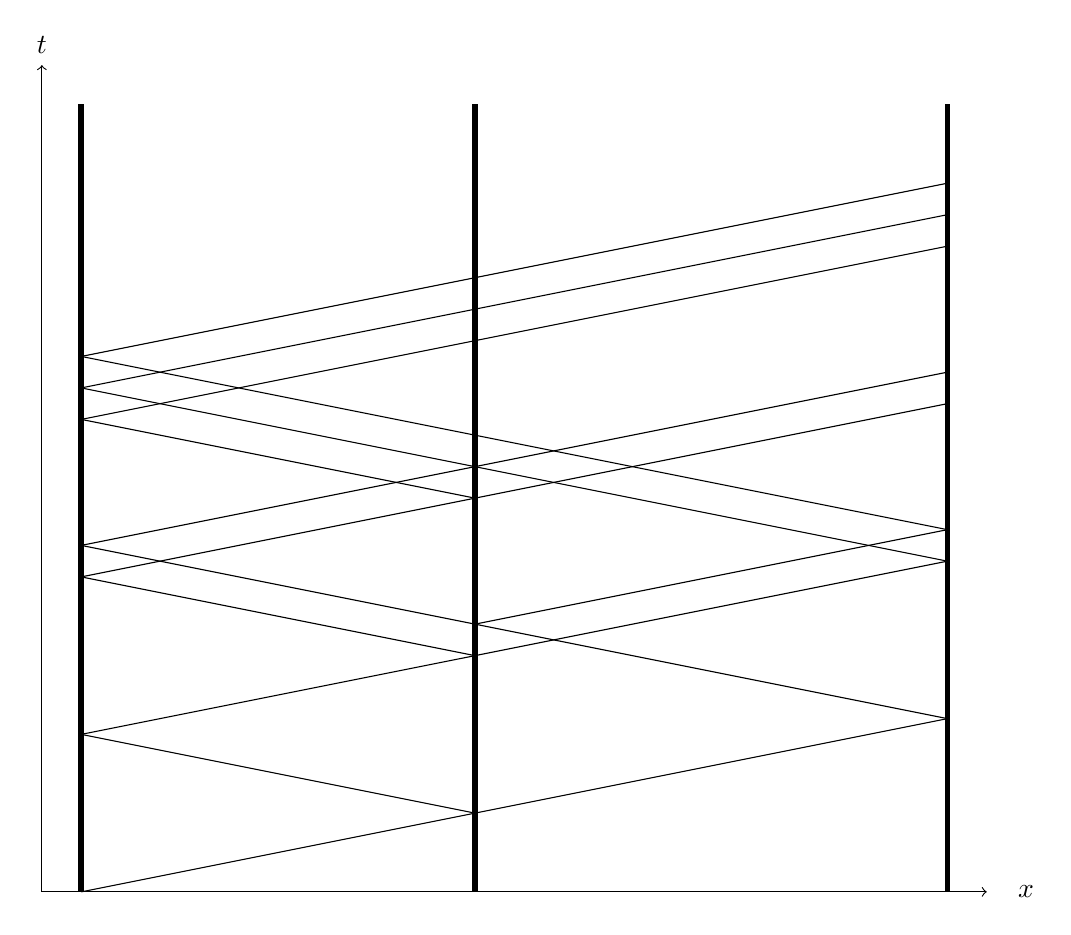
\begin{tikzpicture}
	\draw[line width=2pt] (0,0) -- (0,10);
	\draw[line width=2pt] (11,0) -- (11,10);
	\draw[line width=2pt] (5,0) -- (5,10);
	\draw[->] (-0.5,0) -- node [yshift = 5.5cm]{$t$} (-0.5,10.5);
	\draw[->] (-0.5,0) -- node [xshift = 6.5cm]{$x$} (11.5,0);
	% Linie1
	\draw (0,0) -- (11,1/5*11);
	\draw (11,1/5*11) -- (0,1/5*11*2);
	\draw (0,1/5*11*2) -- (11,1/5*11*3);

	% Linie2
	\draw (5,1) -- (0,2);
	\draw (0,2) -- (11,1/5*11+2);
	\draw (11,1/5*11+2) -- (0,1/5*11*2+2);
	\draw (0,1/5*11*2+2) -- (11,1/5*11*3+2);
	
	%Linie3
	\draw (5,3) -- (0,4);
	\draw (0,4) -- (11, 1/5*11+4);
%	\draw (11, 1/5*11+4) -- (0,1/5*11*2+4);
	
	%Linie4
	\draw (5,5) -- (0,6);
	\draw (0,6) -- (11,1/5*11+6);
	
	\draw (5,1/5*11*2-1) -- (11,1/5*11*2-1+1/5*6);
	\draw (11,1/5*11*2-1+1/5*6) -- (0,1/5*11*2-1+1/5*6+1/5*11);
	\draw (0,1/5*11*2-1+1/5*6+1/5*11) -- (11,1/5*11*2-1+1/5*6+1/5*11*2);
\end{tikzpicture} \\